\chapter{Literature review}\label{ch:LiteratureReview}

\ifpdf
    \graphicspath{{Chapter2_LitReview/Chapter2Figs/PNG/}{Chapter2_LitReview/Chapter2Figs/PDF/}{Chapter2_LitReview/Chapter2Figs/}{Chapter2_LitReview/Chapter2Figs/Classification/}{Chapter2_LitReview/Chapter2Figs/Detection/}{Chapter2_LitReview/Chapter2Figs/Restoration}}
\else
    \graphicspath{{Chapter2_LitReview/Chapter2Figs/EPS/}{Chapter2_LitReview/Chapter2Figs/}}
\fi

\begin{figure}[!] %LitRev_HeisenbergBox_STFT
\centering
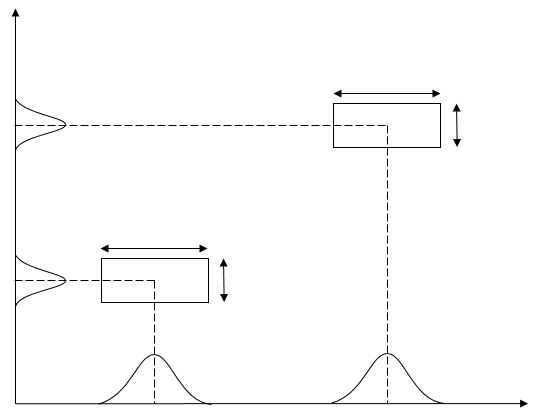
\includegraphics[width=80mm]{LitRev_HeisenbergBox_STFT_2.png}
\begin{picture}(0,0)
\put(-235,170){$\omega$}
\put(-235,122){$\gamma$}
\put(-235,55){$\xi$}
\put(-232,0){0}
\put(-169,-4){$u$}
\put(-67,-4){$v$}
\put(-7,2){$t$}

\put(-220,137){$|\hat{g}_{v,\gamma}(\omega)|$}
\put(-220,35){$|\hat{g}_{u,\xi}(\omega)|$}

\put(-169,75){$\sigma_t$}
\put(-133,57){$\sigma_\omega$}
\put(-150,20){$|g_{u,\xi}(t)|$}

\put(-70,142){$\sigma_t$}
\put(-32,122){$\sigma_\omega$}
\put(-50,20){$|g_{v,\xi}(t)|$}
\end{picture}
\caption{An example of the Heisenberg box illustration and the inherent time-frequency resolution trade-off for the STFT.}
\label{fig:LitRev_HeisenbergBox_STFT}
\end{figure}

\begin{figure}[!] %LitRev_HeisenbergBox_wavelets
\centering
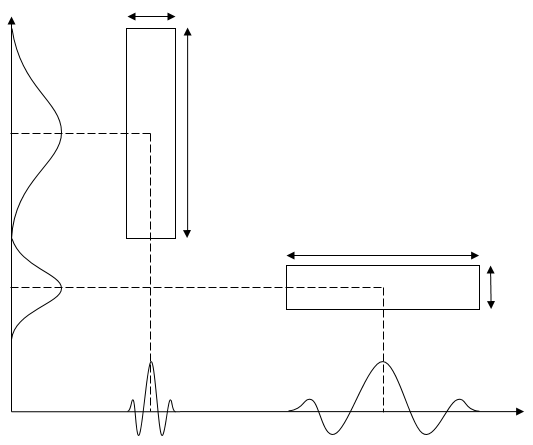
\includegraphics[width=80mm]{LitRev_HeisenbergBox_wavelets_2.png}
\begin{picture}(0,0)
\put(-235,180){$\omega$}
\put(-235,132){$\gamma$}
\put(-235,65){$\xi$}
\put(-232,10){0}
\put(-169,-4){$u$}
\put(-70,-4){$v$}
\put(-7,10){$t$}

\put(-220,140){$|\hat{g}_{v,\gamma}(\omega)|$}
\put(-220,75){$|\hat{g}_{u,\xi}(\omega)|$}

\put(-171,187){$\sigma_t$}
\put(-147,132){$\sigma_\omega$}
\put(-157,30){$|g_{u,\xi}(t)|$}

\put(-70,85){$\sigma_t$}
\put(-18,65){$\sigma_\omega$}
\put(-50,30){$|g_{v,\xi}(t)|$}
\end{picture}
\caption{The Heisenberg boxes for the wavelet transform.}
\label{fig:LitRev_HeisenbergBox_wavelets}
\end{figure}

